\section{Résultats}

\subsection{Twitter}

Le compte twitter totalise un total de 50 abonnés (20/01/2015), en augmentation lente mais constante. On compte parmi ceux-ci des élèves et des anciens élèves, des écoles et des comptes issu du monde universitaire, ainsi que des concours et des professionnels du milieu informatique.


\subsubsection{Ce qui a marché}
\paragraph{Les PICs ASI adoubés une nouvelle fois par norme ISO9001.}
La tournure de la phrase a suscité l'amusement de la communauté et notamment une illustration.
\begin{center}
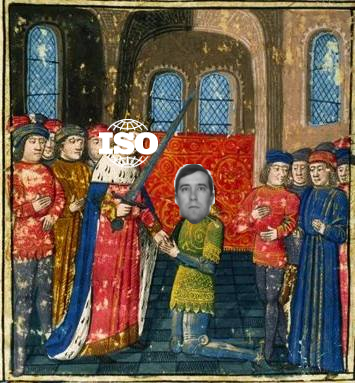
\includegraphics[width=0.45\textwidth]{images/adoubement.png}
\end{center}

\paragraph{Discours de clôture de la \#JSSI et d'anniversaire du département ASI et du \#MasterSSI. \#SequenceEmotion }
Adjoint de ses deux photos, ce tweet a été retweeté plusieurs fois par des intervenant de la JSSI, ce qui a donné une visibilité et a permis de lancer le compte Twitter au terme du livetweet sur la journée.

\subsubsection{Ce qui n'a pas marché}
Il est difficile de dire ce qui ne marche vraiment pas sur Twitter dans le mesure ou le flot continu d'information ne permet pas que tous les postes sucite un engagement particulier. Une étude sur un plus long laps de temps serait nécessaire.
\subsection{Facebook}

La page Facebook totalise un total de 104 abonnés (20/01/2015). La page a connu un énorme pic d'abonnement lors de sa création, essentiellement par les élèves du département, mais plus généralement par les élèves de l'INSA de Rouen. On compte aussi d'ancien élèves de l'INSA, ainsi que leurs proches. Les publications ont atteins au maximum 321 personnes, dont 228 non abonnés.

Les deux graphiques suivant montre un corrélation visuelle imédiate entre la portée de la publication et l'engagement que celle-ci à suscité (mentions "j'aime", partages et commentaires). Il est donc nécessaire de prendre le soin de provoquer cet engagement. 
\begin{center}
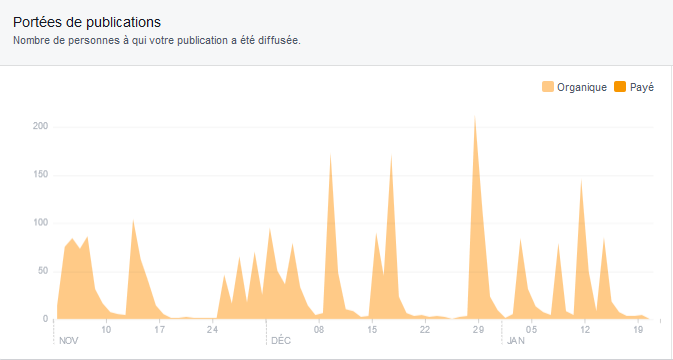
\includegraphics[width=0.90\textwidth]{images/PorteeDesPublication.png}
\end{center}


\begin{center}
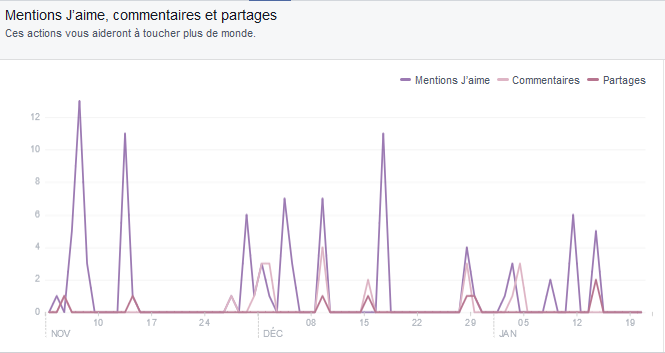
\includegraphics[width=0.90\textwidth]{images/Engagements.png}
\end{center}

La tableau ci-dessous montre les résultats des 10 dernières publications faites sur la page ASI et met en évidence pour chaque publication les résultats de celles-ci.

\begin{center}
	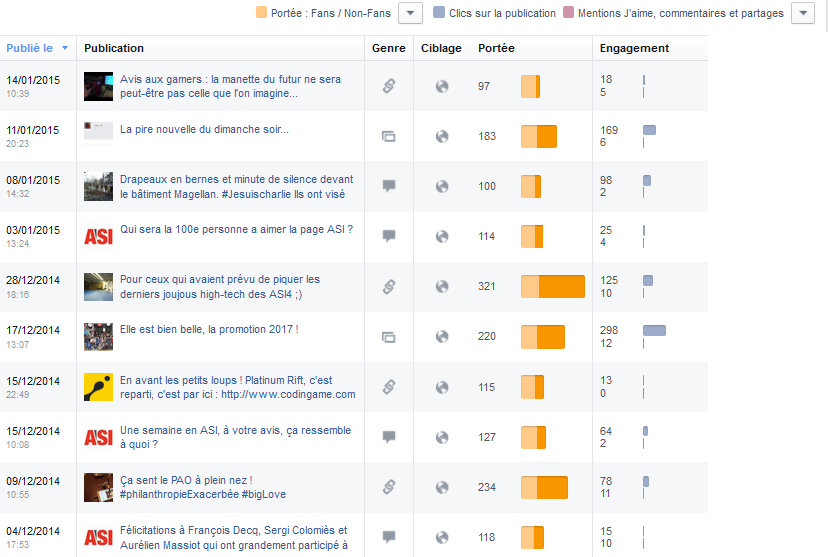
\includegraphics[width=0.90\textwidth]{images/DernierePublication.png}
\end{center}

\subsubsection{Ce qui a marché}
\paragraph{La pire nouvelle du dimanche soir}
Cet publication est une publication simple à but humoristique contenant une phrase courte et incomplète se référent à la photo publiée avec. Elle s'adresse à tous les étudiants qui ont souvent cet angoisse du lendemain de savoir à quelle heure commence la journée du lendemain.
\begin{center}
	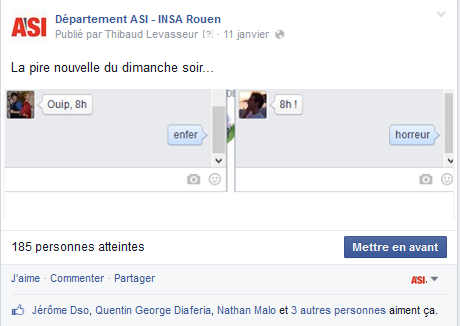
\includegraphics[width=0.90\textwidth]{images/laPireNouvelle.png}
\end{center}

\paragraph{Ca sent le PAO à plein nez !}
Le fameux logiciel de rencontre Tinder qui permet de juger directement sur le physique des gens, est très à la mode chez les jeunes adultes, en raison du tabou qu'il brise. Néanmoins, un internaute a trouvé, à raison que ce n'était pas très sympa pour certains de ne jamais recevoir de "match". Il a donc créé un robot qui apprécie tout le monde en exécutant le « swipe right », grâce a une carte type Arduino et un circuit électrique. Ce statut à la croisée du logiciel et de l'électronique rentre parfaitement dans le cadre de la formation ASI en lui donnant une teinte fine et jeune, ce qui a beaucoup touché les abonnés.


\paragraph{Pour ceux qui avaient prévu de piquer les derniers joujous high-tech des ASI4 }
Nous avons choisi de montrer, avec l'accord de M. Serge Dubois, les vidéos de l'évaluation de combat afin de montrer que même si nous sommes la plupart du temps devant des ordinateurs, nous ne sommes pas pour autant inactif !
Les différentes vidéos de Judo ont suscité un intérêt notable auprès des abonnés de la page Facebook. L'ensemble des vidéos totalise plus de 150 visionnages unitaires et a atteint plus de 300 personnes. C'est certainement le plus gros succès de la page Facebook.


\subsubsection{Ce qui n'a pas marché}
Les postes informatifs ont en général le moins marché et atteignent en général moins de 50 personnes.

\paragraph{Forum Entreprise Étudiant}
Ce groupement de photo était destinés aux ASI4 et 5 en recherche de stage. Néanmoins, comme aucun commentaire ou mention "j'aime" n'est venu alimenter la publication, celle-ci a bien vite disparu des fils d'actualité.

\paragraph{C'est la fête cette année : 30 ans déjà !}
Partage d'une publication de la page Facebook de l'INSA de Rouen, cette publication présente les diverses animations prévu pour l'anniversaire le rapprochement entre l'INSCIR et le groupe INSA.
\subsection{Rayonnement particulier}

Lors des tragiques évènement de début janvier, une minute de silence a été organisé à l'INSA devant les drapeaux près du parking Magellan. Nous avons décidé de couvrir l'événement en partageant le communiqué des présidents d'université ainsi qu'une photo des commémorations le jeudi 8 janvier. 
Le lundi suivant, le cliché est en tête du carrousel des photo des commémorations sur le site http://www.normandie-actu.fr/, crédité à la page Facebook du département ASI de l'INSA de Rouen.
Bien que ce partage soit dû au contexte exceptionnel de la situation, il montre cependant que la presse locale consulte notre page Facebook et/ou notre compte Twitter.

\section{Réalisations graphiques}
	\subsection{Logo ASI}

		\paragraph{}
		

		\begin{center}
			
\includegraphics[width=0.7\textwidth]{images/logo.jpg}
		\end{center}

	\subsection{QRCodes et affiche}

		\paragraph{}
		Les QRCodes, inspirés des codes barres commerciaux, sont un moyen simple et efficace de permettre à des gens d'accéder à un contenu multimédia depuis un smartphone par simple scan de l'image. 
		Nous avons donc créé deux QRCodes : le premier conduisant à la page Facebook, le second au compte Twitter du département.
		
		\paragraph{}
		Nous avons également réalisé une affiche, respectant l'esprit de la charte graphique du groupe INSA, qui contient ces deux QRCodes ainsi que l'adresse du site internet d'ASI.

		\begin{center}
			
\includegraphics[width=0.9\textwidth]{images/affiche.jpg}
		\end{center}
